\section{Type Analyzer}\label{sec:analyzer}

In this section, we explain the detail of the type analyzer of $\tool$. We first
formally define a modified $\ires$ and explain how to perform type analysis
for the modified $\ires$.  Besides, we explain a refinement of type analysis
based on conditions of assertions and branches to increase analysis precision.

\subsection{Intermediate Representation}\label{sec:ires}

$\ires$ is an untyped intermediate representation introduced by \citet{jiset}.
For brevity, we formally define a modified $\ires$ as follows:
\[
  \begin{array}{lr@{~}r@{~}l}
    \text{Instructions}
    & \inst &::=&
    \kwlet \; \x = \expr \mid
    \kwlet \; \x = \kwrl \expr \; \expr^* \kwrr \mid
    \kwassert \; \expr \\

    &&\mid&
    \kwif \; \expr \; \lab \; \lab \mid
    \kwreturn \; \expr \mid
    \refer = \expr \\

    \text{References}
    & \refer &::=&
    \x \mid
    \refer \kwsl \expr \kwsr \\

    \text{Expressions}
    & \expr &::=&
    \tname \kwcl [\x \kwarrow \expr]^* \kwcr \mid
    \expr: \ty \mid
    \refer \kwexists \mid
    \expr \bop \expr \mid
    \uop \expr \mid
    \refer \mid
    \const \mid
    \prim \\

    \text{Primitives}
    & \prim &::=&
    \undefval \mid \nullval \mid \bool \mid
    \num \mid \bigint \mid \str \mid \symb \\

    \text{Types}
    & \ty &::=& \tname \mid \tjs \mid \tprim \mid
    \undefval \mid \nullval \mid \tbool\\

    &&\mid&
    \tnumeric \mid \tnum \mid \tbigint \mid \tstr \mid \tsymb \\
  \end{array}
\]
A modified $\ires$ program $\prog = (\getlab, \nextlab)$ is a pair of two finite
mappings. The getter mapping $\getlab: \labset \finmap \instset$ represents
instructions attached to labels, and the next mapping $\nextlab: \labset \finmap
\labset$ denotes next labels. A label $\lab \in \labset$ denotes a program
point.  An instruction $\inst$ is a variable declaration, a function call, an
assertion, a branch, a return, or an reference update.  Each invocation of an
abstract algorithm in ECMAScript is compiled to a function call instruction with
a newly introduced temporal variable.  We represent loops using branch
instructions with cyclic pointing of labels in the next mapping $\nextlab$.  A
reference $\refer$ is a variable $\x$ or a field access $\refer \kwsl \expr
\kwsr$.  An expression $\expr$ is a record, a type check, an existence check, a
binary operation, a unary operation, a reference, a constant, or a primitive,
which is either $\undefval$, $\nullval$, a Boolean $\bool$, a Number $\num$, a
BigInt $\bigint$, a String $\str$, or a Symbol $\symb$.

\begin{figure}
  \centering
  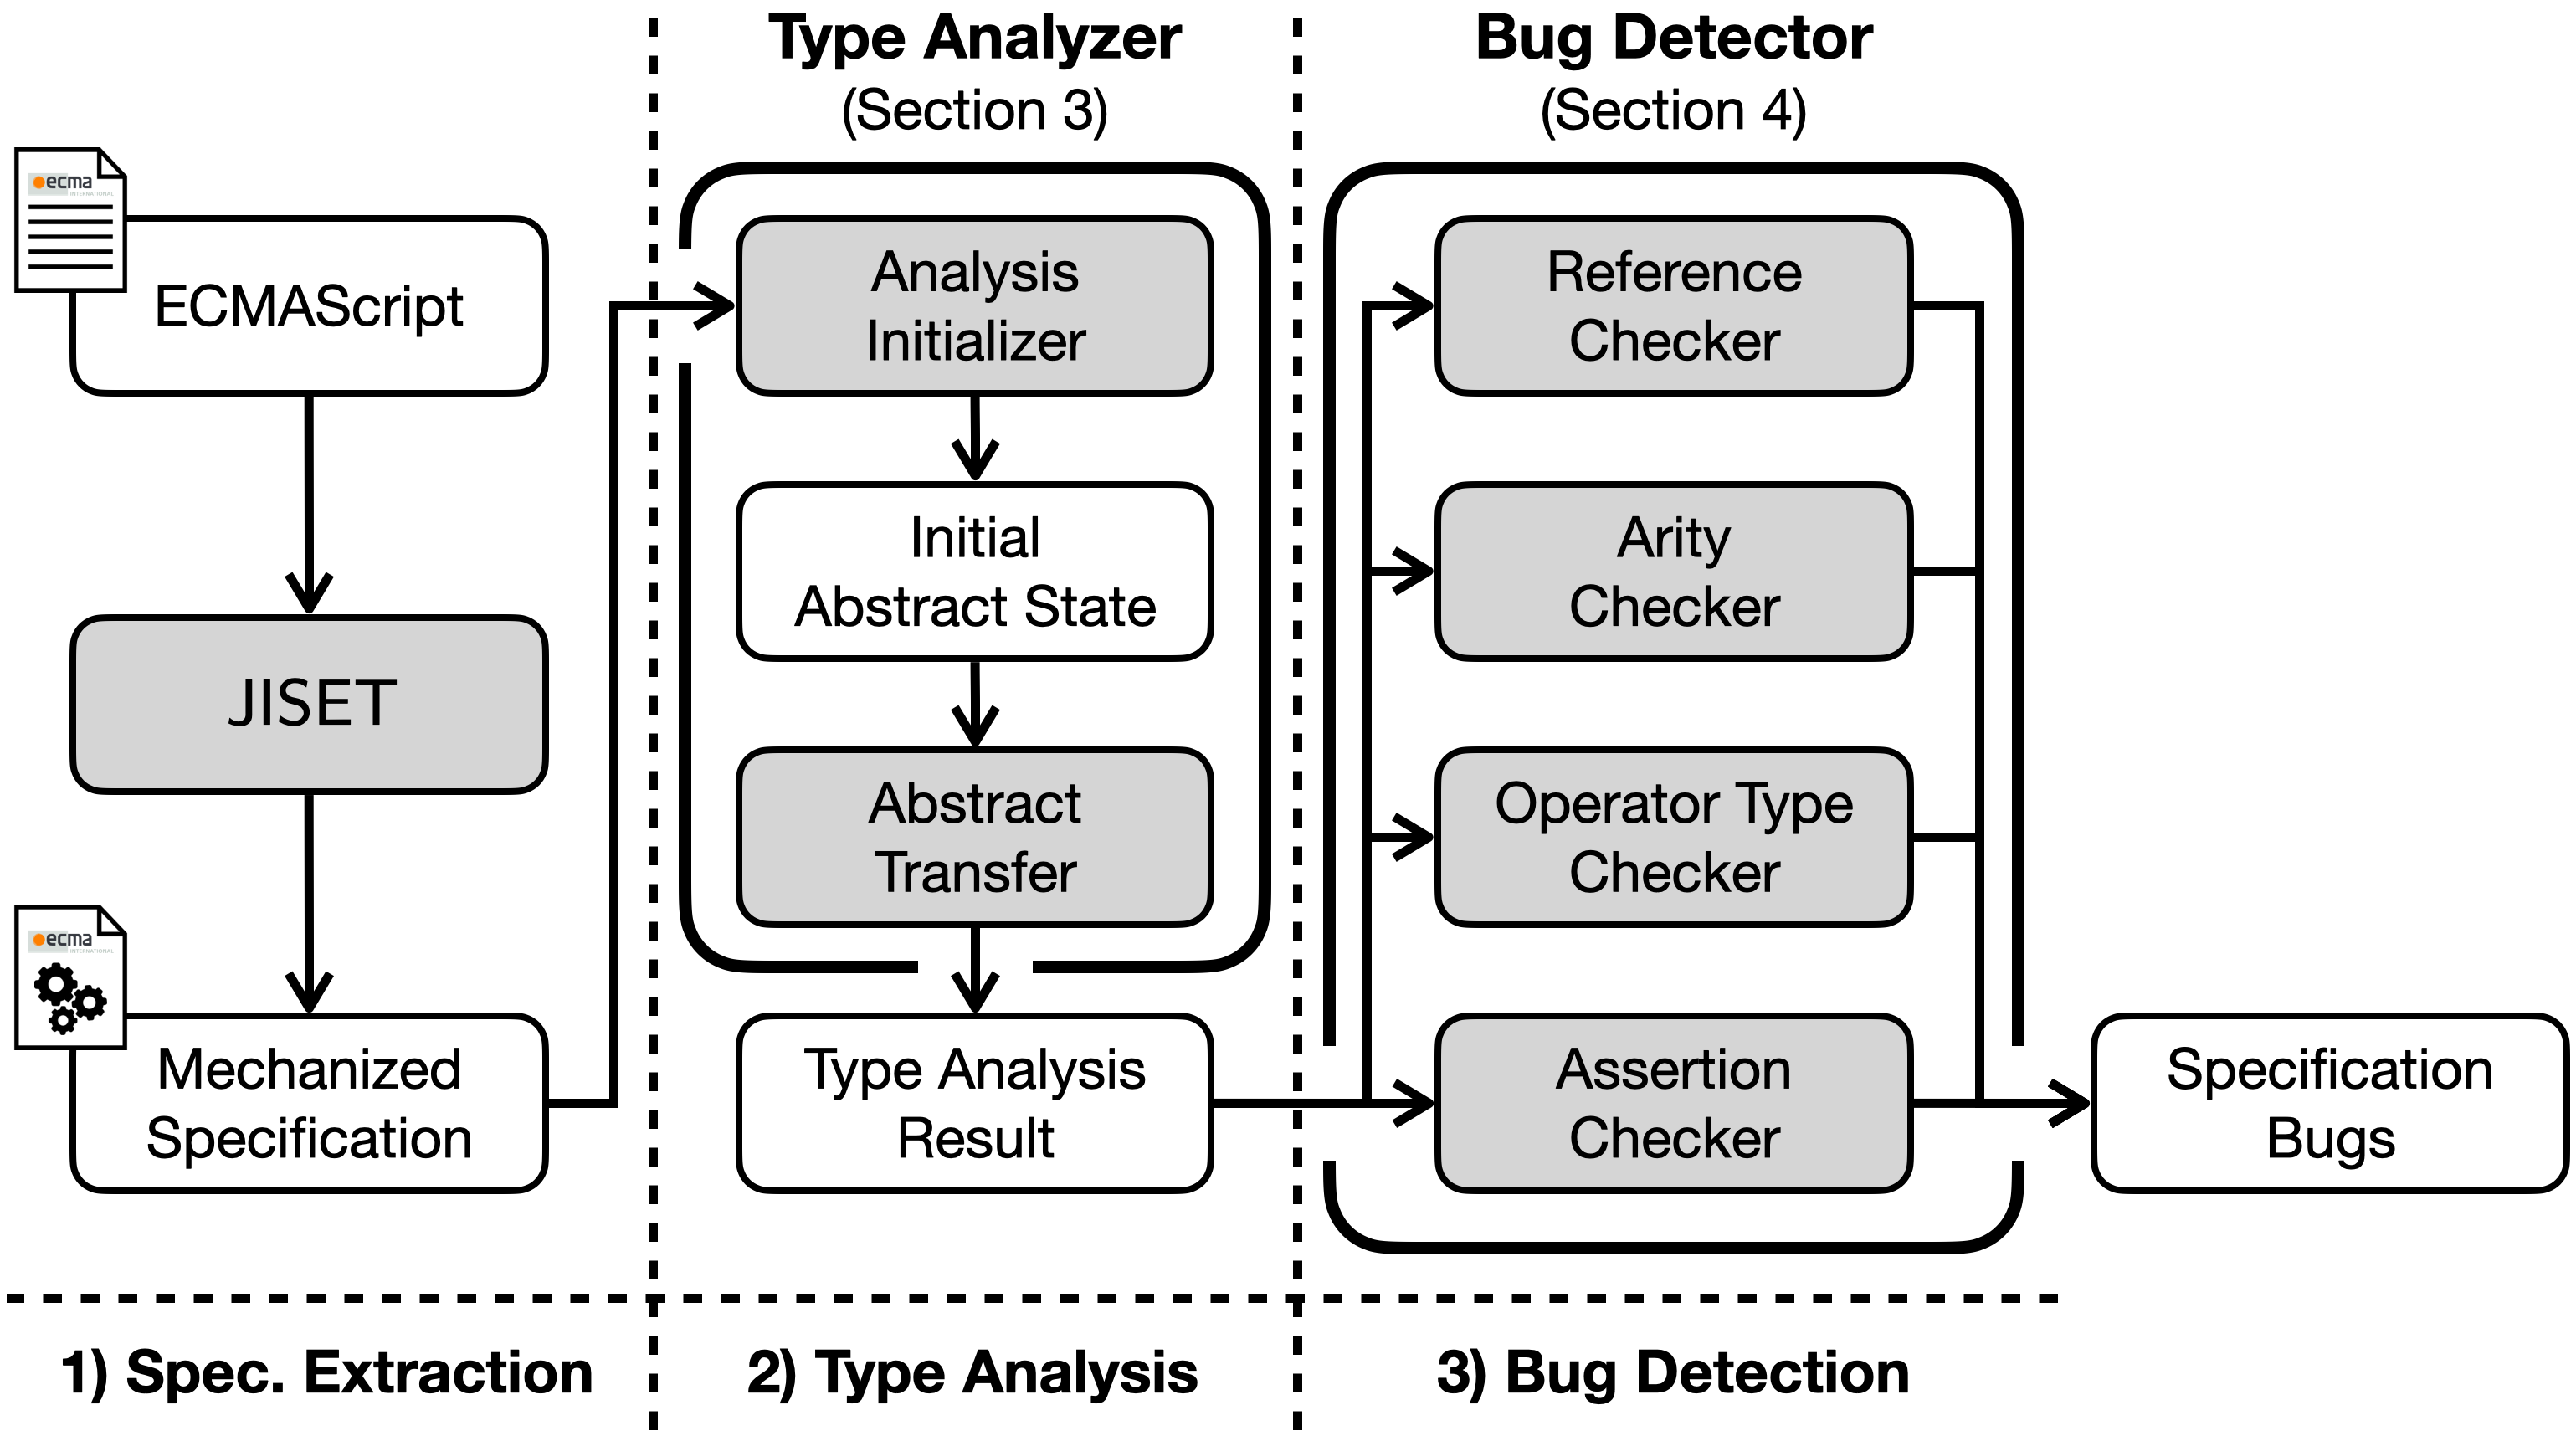
\includegraphics[width=0.48\textwidth]{img/overall}
  \vspace*{-1.5em}
  \caption{The subtype relation $\subtype$ between types.}
  \label{fig:subtype}
  \vspace*{-1.5em}
\end{figure}

A type $\ty \in \tyset$ is a norminal type $\tname$ or a pre-defined type;
$\tjs$ denotes JavaScript values, $\tprim$ primitives, $\tnumeric$ either Number
or BigInt values, and $\tnum$, $\tbigint$, $\tstr$, and $\tsymb$ denote Number,
BigInt, String, and Symbol values, respectively.  A norminal type $\tname$ is a
production name for ASTs or a record type name used in abstract algorithms.  The
subtype relation $\subtype \subseteq \tyset \times \tyset$ between types is
described in Figure~\ref{fig:subtype}; the directed edge from $\ty'$ to $\ty$
denotes $\ty' \subtype \ty$ and the relation is reflexive and transitive.  For
example, \inred{name and subtype example using 14.1.19 in Figure 2}.  Based on
this subtype relation, a type check expression $\expr: \ty$ checks whether the
evaluation result of $\expr$ has a type $\ty' \subtype \ty$.  


\subsection{Type Analysis}\label{sec:analysis}

\subsection{Refinement}\label{sec:refine}
